\section{Laboratory}
This project was run under a GNU/Linux distribution in one of the personal computers of the student.
Said computer has 20GB of RAM, an \textit{i5-2500k} processor and about 500GB of free disk storage for this project (of which 100GB were of Solid State Disk).
\linej
\linej
Hosting services were considered but discarded, because their biggest advantage would be to be able to work on this project anywhere (since the only user is the student). This is something that can be achieved in a home computer with port redirection and either knowing the external IP of the router or using a naming service, but in this case there was no need to connect from the outside.

\subsection{Virtual machines}
VirtualBox was chosen as the host program of the virtual machines because it was the one the student had the most experience with.
\linej
This laboratory consist of multiple virtual machines, that represent:
\begin{itemize}
	\item An enterprise domain of Windows computers, named \textbf{Wazuh.local}, managed by Windows' Active Directory:
		\begin{itemize}
			\item Windows Server 2019, as Domain Controller of the Active Directory.
			\item Windows Server 2019, as a SMB file server.
			\item Windows 10, as a basic workstation.
		\end{itemize}
	\item The Wazuh server: A CentOS 7. As mentioned before in \ref{singlehost}, we are using a single server to host both the Wazuh manager and the ELK stack.
	\item An offensive security box: In this case with Kali Linux. This is used to access the Windows boxes in some of the attacks.
\end{itemize}

\begin{figure}[H]
  \centering
	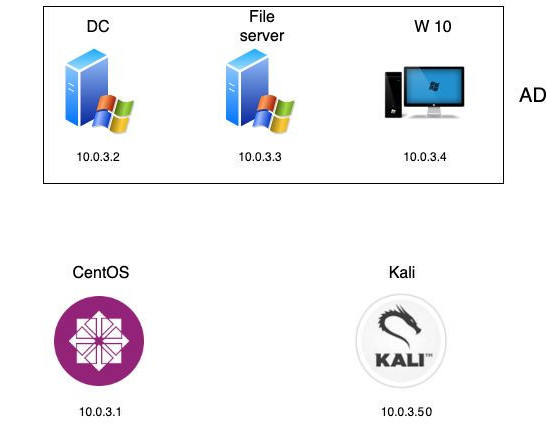
\includegraphics[width=\textwidth]{figuras/virtual_machines.jpg}
	\caption{Virtual machines in the project}
\end{figure}
\linej
Every machine has two network interfaces, one for the internal network (10.0.3.0) and another for accessing the internet connection of the host.
Each of the Windows boxes have a Wazuh agent installed, that reports to their manager (server) in the CentOS box.
All the ruleset changes and log processing was done directly on the CentOS machine.
\linej
\linej
Most of the time only the DC and the CentOS machine were powered on, but when all of them were being used at the same time they consumed about 12GB of RAM. Leaving aside booting, they did not affect performance in a perceptible way, either one to each other or to the host.
\linej
\linej
Snapshots were taken when significant changes were made, like relevant installation or configuration. Then the virtual machines with their snapshots were copied to a couple of external disks as backup. At the end of the project near 60 snapshots were taken and the virtual machines with their snapshots were using about 160GB of disk space.


